\scanpage{47}
\begin{center}- 15 -\end{center}
\hfill n$^\circ$ 276

linéaire des $\alpha_{rs}X^r$ si $r\leq n$, et des $\alpha_{ns}X^r$ si $r>n$, d'où évidemment notre assertion.

(La démonstration précédente ne semble pas présenter d'avantage très décisif par rapport à la démonstration classique \ldots)

\uline{Corollaire 1} -- \uline{Soit} $K$ \uline{un corps} ; \uline{l'anneau de polynômes} $K[X_1,\ldots,X_r]$ \uline{est noethérien}.

On raisonne par récurrence sur $r$.

\margin{?}
\uline{Corollaire} 2 -- \uline{Soit} $A$ \figure{\begin{tikzpicture}[baseline=(n.base)]\node[draw,ellipse,inner sep=2pt] (n) {\uline{un anneau commutatif noethérien}};\end{tikzpicture}}. \uline{L'anneau de séries formelles} $A[[X]]$ \uline{est noethérien}.

Filtrons $A[[X]]$ par les puissances de l'idéal $(X)$ ; on obtient un anneau séparé et complet (Corollaire de la Proposition 5) ; or l'anneau gradué associé, isomorphe à $A[X]$, est noethérien ; donc $A[[X]]$ est noethérien en vertu du corollaire 2 de la proposition 7.

\uline{Corollaire} 3 -- \uline{Soit} $K$ \figure{\begin{tikzpicture}[baseline=(n.base)]\node[draw,ellipse,inner sep=3pt] (n) {\uline{un corps}};\end{tikzpicture}} ; \uline{l'anneau de séries formelles} $K[[X_1,\ldots,X_r]]$ \uline{est noethérien}.
\margin{\figure{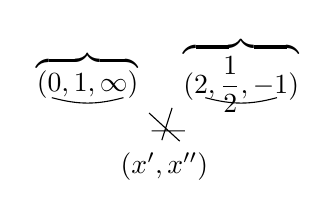
\begin{tikzpicture}[scale=.65]\node at (-1.5,1.1) {$\overbrace{(0,1,\infty)}$};\node at (1.5,1.1) {$\overbrace{(2,\frac12,-1)}$};\node at (0,-.7) {$(x',x'')$};\draw (-.25,0)--(.4,0) (-.05,-.18)--(.15,.45) (-.3,.35)--(.3,-.2);\draw (-2.2,.65) to[bend right=15] (-.8,.65);\draw (.8,.65) to[bend right=15] (2.2,.65);\end{tikzpicture}}}

Cela résulte du corollaire précédent par récurrence sur $r$.

Le corollaire 2 résulte aussi du suivant :

\uline{Corollaire} 4 -- \uline{Soient} $A$ \uline{un anneau commutatif et} $\mathrm m$ \uline{un idéal de} $A$. \uline{Supposons} $A/\mathrm m$ \uline{noethérien}, $\mathrm m$ \uline{à engendrement fini}, \uline{et} $A$ \uline{séparé et complet pour la topologie} $\mathrm m$-\uline{adique}. \uline{Alors} $A$ \uline{est noethérien}.

En effet, si $\mathrm m$ est engendré par des éléments $x_i$ en nombre fini dont nous noterons $\bar x_i\in G_1(A)$ les formes initiales, il est clair que tout élément de $G(A)$ est un polynôme en les $\bar x_i$, à coefficients dans l'anneau $G_0(A)=A/\mathrm m$ ; $G(A)$ est donc noethérien, d'où le résultat.

\uline{Corollaire} 5 -- \uline{Soit} $g$ \uline{une algèbre de Lie sur un anneau commutatif noethérien} $K$. \uline{L'algèbre enveloppante de} $g$ \uline{est un anneau noethérien (à gauche et à droite)}
\mspage{46}
